\begin{quote}
This conversational piece invites you to engage in a journey to create
your own learning space. You'll find many points of entry that allow you
to affectd emerging structure. Reciprocal mentoring can create a ripple
effect for those who follow.
\end{quote}

\subsection{The Guiding Strategy:}\label{the-guiding-strategy}

In his \href{http://peeragogy.org/case-study-5ph1nx/}{Peeragogical Case
Study} David Preston states:

\begin{quote}
\emph{Peeragogical interaction requires refining relational and topical
critique, as well as skills in other ``meta'' literacies, including but
not limited to critical thinking, collaboration, conflict resolution,
decision-making, mindfulness, patience and compassion.}
\end{quote}

A
\href{http://en.wikipedia.org/wiki/Self_Organised_Learning_Environment}{Self-Organizing
Learning Environment}, or SOLE, with a living structure accomplishes all
of these outcomes, or David's ``meta-literacies,'' simultaneously. An
authentic problem and/or project based activity in a connected learning
environment includes diverse learners in diverse ways by empowering all
learners as peers.

This provides the authentic learning environment with which to design a
SOLE. SOLEs are everywhere. How have we evolved as a species, if not
through self-organizing? A conversation between strangers is self
organizing, each learning about something or each other. The spaces
around people conversing is also an environment, though not explicitly a
learning one. 

While we are always self-organizing to learn or accomplish

\clearpage
\begin{vplace}[0.5]
\noindent 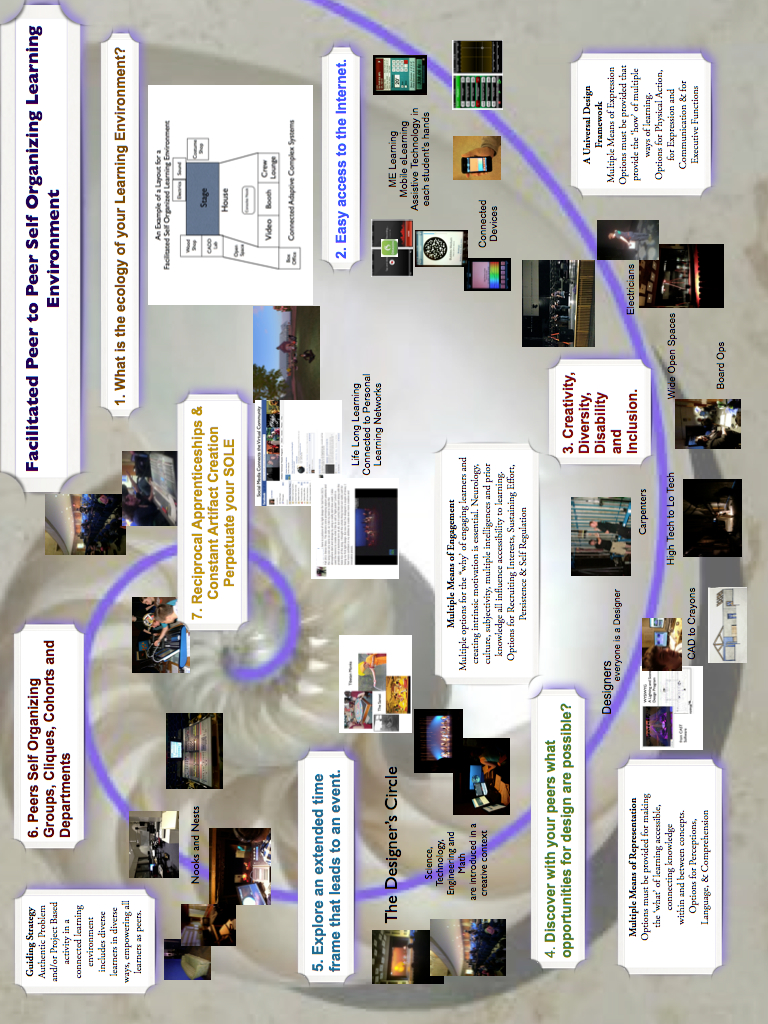
\includegraphics[width=\textwidth]{../pictures/sole-l.jpg}
A visualization of the facilitated peer to peer SOLE, full-size
at \url{http://goo.gl/7StkJK}
\end{vplace}
\clearpage

\noindent things, one place that SOLEs do not always exist are in
learning institutions. In many educational institutions, our learning
environments are predominately organized by the teacher, curriculum,
or society. How can we nurture peer to peer learning environments to
organize? How does the role of the teacher differ in a SOLE? In what
ways can we unite that fundamental, passionate human characteristic of
curiosity and self-organizing back into our Learning Environments?

The model that \href{http://sugatam.wikispaces.com/}{Sugata Mitra}
{{[}2{]}} is experimenting with gives us some scaffolding to create one
ourselves. This is the goal of his
\href{http://www.ted.com/pages/sole_toolkit}{SOLE Tool Kit} (3).
Sugata's kit is directed towards children between 8 and 12 years old. I
was wondering if there is a way to make it more universal in its
application. How can I apply it to my situation? How is a SOLE different
in the context of peer to peer learning? This chapter of the Handbook
uses Sugata's model as a doorway into our understanding a SOLE approach
to peer to peer learning. Its three key components are: learners,
context and project. I find the discussion needs to integrate what we
are learning about diverse learners into a
\href{http://www.udlcenter.org/aboutudl/udlguidelines}{Universal Design
for Learning} {{[}4{]}} context. After all, we cannot take for granted
who the peers are in the SOLE. Equally, the context, the learning
environment (LE) must be as deeply considered as the learners
participating. As a learning designer, I am also seeking more clues
about the living structure of a well crafted SOLE.

\subsection{Centers within the Center}\label{centers-within-the-center}

SOLEs exist in a particular context. Take Sugata's
\href{http://www.ted.com/talks/sugata_mitra_shows_how_kids_teach_themselves.html}{hole
in the wall} {{[}5{]}} experiment. The parameters of the environment of
a computer embedded in a wall in India are very specific. Sugata's act
was to design a project in order to facilitate a process within that
environment. The elements he introduced were a touch screen computer
embedded in a wall with specific software. Sugata has abstracted this
design into a Tool Kit. He speaks of `Child Driven Learning',
intrinsically motivated learning with the curiosity to learn something
in particular. As a learner-centric peeragogy, SOLEs are emergent,
bottom up, seeking to answer: How do we design a project (or phrase a
problem) that ignites a learner's passion?

A SOLE is a facilitated learning environment (LE) that can nurture
learner-driven activity. For instance, in the Hole in the Wall example,
the design is the context of the wall, the street, the neighborhood
--and the facilitation is the touch screen monitor in the wall. They are
brilliantly united. In this sense it is an intentional, self-aware
learning environment. The Wall's computer is a strange foreign object
that anyone would have to figure out how to take advantage of. But this
is not in the classroom, or in the `school.' It is an informal LE. Just
like
\href{http://www.academia.edu/1137269/Game-based_Learning_and_Intrinsic_Motivation}{learning
a game} {{[}6{]}}, there is an entire ecology that surrounds you. This
is very much a systemic approach. The context is facilitated explicitly
(your design of the SOLE), but also implicitly in the
\href{http://en.wikipedia.org/wiki/Hidden_curriculum}{hidden curriculum}
{{[}7{]}} that defines your LE. 

Above is the layout of the
\href{http://www.scribd.com/doc/181089012/Transformed-Learning-Environment-Analysis}{transformed
learning environment} {{[}8{]}} I explored to work around the hidden
curriculum of the traditional classroom. The LE has a tremendous, if not
\href{http://scholar.lib.vt.edu/theses/available/etd-09232007-220306/unrestricted/SElmasryETDbodytext.pdf}{overwhelming
influence, on learning} {{[}9{]}}. The first step in connected learning
is to reconnect to the environment around us. For me, the primary
context of my LE is a performing arts center at a small rural liberal
arts college. The Performing Arts Center is a Center within the context
of the college and community. A diversity of spaces within the facility
are inhabited: small and cozy, large and public, technology embedded
everywhere, all focused on the project based learning that emerges
producing a performance. I stay away from a formal classroom as much as
possible. These spaces are Centers within the Center,
`\href{http://nourdiab.wordpress.com/2011/02/23/the-theories-of-christopher-alexander/}{loosely
connected adaptive complex systems}' {{[}10{]}} within themselves, just
like people. I believe that the possibility of a SOLE emerging as a
living structure seems to depend on the correct types of complex systems
engaged in the LE.

What is the role of the internet in your design? Mitigating inequalities
and accommodating diverse learners are somewhat assisted by access to
the internet. But it is the immediate,
\href{http://www.wordstream.com/blog/ws/2013/10/02/just-in-time-information-hacks}{just-in-time
learning} {{[}11{]}} that makes free and open access to the world wide
web so important in a SOLE. Wireless is available throughout this LE.
Nooks and lounges, interconnected, but separate rooms, provide lots of
places for collaboration or solitary work, for staying connected or
hiding out. In a UDL vision of a facilitated peer to peer SOLE,
technology is integral to the design. In the case of my LE, with the use
of digital audio, multi-media, database management, robotic lighting and
\href{http://en.wikipedia.org/wiki/Dichroic_filter}{dichroic} {{[}12{]}}
colors, learners are accustomed to accessing and augmenting reality with
technology: allowing learners to access their social media is part of
their content creation.

Do we start our SOLE as peers? Peer to peer assumes your participants
are peers--especially you, the facilitator. There needs to be enough
diversity and complexity to include all learners, engendering a
\href{http://www.cast.org/library/UDLguidelines/}{Universally Designed
Context} {{[}13{]}}. What is the role of diversity in peer to peer SOLE
building? How are diverse learners peers? In my LE, I discovered 70\% of
my learners have learning challenges. I know my LE is not unique in this
regard. I have to facilitate a SOLE design that is inclusive. This is in
contradistinction to commonality, yet this diversity is what we crave,
for creativity and innovation, for deep learning to occur. Crafting your
SOLE using multiple means of representation, expression and engagement
empowers learners to be peers. A diverse learning environment,
supporting diverse learning styles and diverse learners, supports a
complex project based SOLE. But there are many SOLEs within the SOLE
since learning is occurring on many levels with each student and within
each group. We do not all get the same thing at the same time. Learning
outcomes are diverse, emergent, serendipitous.

What type of project, problem or event will focus your efforts? Either a
{[}learner generated syllabus
\href{http://www.theatreprof.com/2011/active-learning-student-generated-syllabus/}{}14{]}
may emerge from the SOLE, or a
\href{http://usergeneratededucation.wordpress.com/}{user generated
education} {{[}15{]}} within a specific context may answer this
question. Ownership and leadership emerge when learners can apply their
creativity and/or authentically assist each other in a common goal.
Opportunities to design and modify even small things will draw learners
into a project. The more they must rely on each other, collaborate and
share their creativity, their designs and actualization--the more they
work together as peers. The spaces in your LE are most likely already
designed and built to accommodate the purpose of the facility in the
context of the college or school. We cannot really redesign the actual
space, but we can redesign many aspects. We can look for designs within
it. Being able to design your own space, or project, is critical to
taking ownership of your learning and experiencing the consequences. As
learners mature and look for ways to be more involved, I suggest they
redesign the shop, the repertory lighting plot, or the procedures of
their department and/or SOLE overall. Exchanging roles as designer also
stimulates peer interaction. Why not integrate design and design
thinking? In my context, lighting, scene, costume and sound design are
interconnected opportunities. Along with accompanying technology, every
opportunity is used to nurture empathy, creativity, rationality and
systems thinking. Integral to the learner generated syllabus or project
design should be continuous artifact creation. A great place to start
the design process and to begin to generate content is by using a
virtual world.

Constant content creation can integrate assessment into your SOLE. It is
the quality of the artifacts created along the way that reveals the
success of your SOLE. Media that chronicles a journey through time,
created by each learner, reveals the depth of participation. It is
nearly impossible to cheat. The learner expresses their comprehension in
the types and extent of artifact creation.

As the facilitator, I look for opportunities to introduce the
unexpected, bigger questions, deeper considerations, along the way. For
example, in the context of my LE, one of the events feature Tibetan
Monks. They bring a counterpoint to the inflated egos and cult of
personality which is prevalent in our context. The SOLE Plan is
extended. It can happen over a much longer amount of time than one class
or one day. The actors rehearse for weeks, as the design team designs,
giving time for: research, absorption, misleads, mistakes, correction
and reflection. A SOLE needs time and persistence to generate artifacts,
documentation and experiences of the project and virtual worlds are an
excellent way to extend time and space synchronously and asynchronously.

Sugata emphasizes the Big questions. We do not always know what they
are. A focus? A goal? A product? And the event? That should be decided
with the group. The learners intuit the direction that leads to deep
engagement and the bigger questions. I try and leave it ambiguous,
suggesting some of the things they might encounter. Facilitating the
SOLE in this context, we face endless questions connected to the
specific LE, to all the imaginary scenarios, Herculean tasks and
questions-- like building castles, programming a digital sound console,
troubleshooting robotic lighting instruments, how to make the illusion
of fire or, even, who killed Charlemagne? The Box Office is an example
of an informal SOLE that has emerged recurrently over time. I have
noticed that its vitality depends on the characters and the ebb and flow
of learners entering the group or graduating.

The physical space is a small, windowless and often damp room with a couple
of couches and a desk with a computer squeezed in. My very own `Hole in
the Wall' experiment. The bottom of the door can remain closed, while
the top is open, like a stable. Primarily the students are paid to be
there, answering the phone, reserving tickets, greeting patrons and
managing the Box Office and the Front of the House. In the SOLE, this
subtle inversion of the institutional value proposition turns `work
study' into studying work. This is an informal LE nested within the
context of the formal institution and the wider LE: a center within a
center. Some semesters there are business majors working their way up
the job ladder: Usher to Assistant Front of House Manager, to Assistant
Box Office Manager, to Box Office Manager. Sometimes this takes 4 years,
sometimes it happens in a semester or two. It is a recursive SOLE that
differs as the interests and skills of the students who inhabit the
space change. As the current manager puts it, the Box Office is a
`constantly evolving puzzle.'

This example of a SOLE in an informal LE is similar to the other types
of SOLE's that occur within a facilitated LE. The learner's interact as
reciprocal apprentices, leaning on one another to solve challenges and
problems. Groups are self-selective, this type of work suits their
temperament and interests, or time. This cohort is almost a clique,
attracting their boyfriends and girlfriends. They begin initiatives,
re-design the lobby for crowd control, redecorate and rearrange the
space constantly, decide their schedules and split up responsibility.
Everyone is always training everyone, because the environment turns over
each semester. It is explicitly an informal LE. The workers are
students. This inverts the usual state of affairs, where essentially
they are being paid to learn, though they may not even be aware of it.
Occasionally, the learning experience resonates deeply with them. A
number of them have used the experience to leverage jobs that parallel
their interests, or get them started on their careers.

Job titles, roles of responsibility, are often problematic in a SOLE.
The bottom line is that as peers we are all equal and at certain times
everyone is expected to do everything regardless of their roles. Titles
go to people's heads. But this is part of the experience. Keep the
titles moving, change it up when things get bottlenecked over
personalities. Sometimes I create duplicate positions, Assistants of
Assistants. and Department Heads. The Apprenticeship model is at play
but in a new way in a SOLE. There are peers and there are peers. As
power struggles emerge, some like-to-like grouping occurs. The role of
the facilitator becomes mediator. The emergent epistemology of abundance
and connected learning asks for a multitude of `experts.' In the same
way, leadership can be distributed, flowing as varying needs arise.

The experience of practicing leadership skills and encountering all the
variables of working with diverse folks quickly gives feedback to us if
this is a helpful role for this person. It is messy sometimes, and there
are conflicts. After a few events, they learn how to manage a Box
Office, dealing with patrons, emergencies, complaints and bag check.
They confront the larger peer group, the student body, with authority
and empathy. They are very proud of their jobs and make their own name
tags with titles. A hierarchy gives them rewards that they have been
trained to expect from years in school. It is another way of developing
intrinsic motivation and challenges them to interact with their peers
authentically.

As facilitator, I try to leave them alone as much as possible. The
context has been created, the computer in the wall is on a desk.
Extending the design of your SOLE contributes to its living structure. I
have used
\href{http://community.telecentre.org/profiles/blogs/facebook-as-a-supplemental-lms}{Facebook
as a Supplemental LMS} {{[}16{]}} since 2007 because this is where my
students are and it allows them to control the structures of groups
emergently. The learners create the groups as they are relevant. The
facilitator does not. Usually they invite me in! For now, Facebook
aggregates the learning community that the SOLE inspires as learners
become leaders, establish connections with each other and mentor
newbies. This activity is integrated into artifact creation, `comments'
and documentation of their personal learning journey. Facebook becomes a
precursor for their portfolios, and in some cases, it is their
portfolio.
\href{http://starwars.wikia.com/wiki/Reciprocal_apprenticeship}{Reciprocal
Apprenticeships} {{[}17{]}} occur in the dynamic of collaboration among
peers. Continuity in time beyond the event horizon is accomplished by
these relationships. Peers nurture one another along the shared learning
journey that the SOLE provides. As facilitator and designer, you are,
most of all, in a reciprocal relationship with the other learners. This
is the essence of being a peer, an interaction that respects what each
of us brings to the experience.

\subsection{A review}\label{a-review}

\begin{quote}
\textbf{Sugata Mitra}: It is great to see the thinking that has gone
into taking the idea of a SOLE forward. To my mind, SOLEs are quite
experimental at this time and efforts such as these will provide
invaluable data. I look forward to this. I notice that most of the
important design features of a SOLE are incorporated into the article. I
repeat them anyway, just to emphasise:

\begin{enumerate}
\def\labelenumi{\arabic{enumi}.}
\item
  Large, publicly visible displays are very important, this is what
  resulted in the surprising results in the hole in the wall experiments
  and subsequent SOLEs for children in England and elsewhere.
\item
  The absence of unnecessary people in the learning space, no matter who
  they are; parents, teachers, principals, curious adults etc.
\item
  Free, undirected activity, conversation and movement.
\item
  A certain lack of order: I must emphasise that `Self Organised', the
  way I use it does not mean `organising of the self'. Instead it has a
  special meaning from the subject, Self Organising Systems, a part of
  Chaos Theory. The SOLE should be a space at the `edge of chaos',
  thereby increasing the probability of the appearance of `emergent
  order'.
\end{enumerate}

\subsection{References}\label{references}
\end{quote}

\begin{enumerate}
\def\labelenumi{\arabic{enumi}.}
\item
  Preston, David (2014).
  \href{http://peeragogy.org/case-study-5ph1nx/}{Case Study: 5PH1NX}
  (pp. --, this volume).
\item
  \href{http://sugatam.wikispaces.com/}{About Sugata Mitra}, on
  Wikispaces.
\item
  \href{http://www.ted.com/pages/sole_toolkit}{The SOLE Toolkit}, on
  TED.com.
\item
  National Center for Universal Design for Learning,
  \href{http://www.udlcenter.org/aboutudl/udlguidelines}{Universal
  Design for Learning Guidelines}.
\item
  Sugata Mitra (2010).
  \href{http://www.ted.com/talks/sugata_mitra_the_child_driven_education.html}{The
  child-driven education}, TED.
\item
  \href{http://www.academia.edu/1137269/Game-based_Learning_and_Intrinsic_Motivation}{Game-based
  Learning and Intrinsic Motivation by Kristi Mead}.
\item
  \href{http://en.wikipedia.org/wiki/Hidden_curriculum}{Hidden
  Curriculum}, on Wikipedia.
\item
  \href{http://www.scribd.com/doc/181089012/Transformed-Learning-Environment-Analysis}{Transformed
  Learning Environment Analysis}, by Jan Herder (on ScribD).
\item
  Elmasry, Sarah Khalil (2007).
  \href{http://scholar.lib.vt.edu/theses/available/etd-09232007-220306/unrestricted/SElmasryETDbodytext.pdf}{Integration
  Patterns of Learning Technologies}. IRB\# 05-295-06.
\item
  Curious:
  \href{http://nourdiab.wordpress.com/2011/02/23/the-theories-of-christopher-alexander/}{In-Forming
  singular/plural design, The Theories of Christopher Alexander}.
\item
  \href{http://www.wordstream.com/blog/ws/2013/10/02/just-in-time-information-hacks}{Overwhelmed
  with Blog Tips? Hack Learning with Just In Time Information}, on
  Wordstream.com.
\item
  \href{http://en.wikipedia.org/wiki/Dichroic_filter}{Dichroic Filter},
  on Wikipedia.
\item
  \href{http://www.cast.org/library/UDLguidelines/}{UDL Guidelines} on
  cast.org.
\item
  \href{http://www.theatreprof.com/2011/active-learning-student-generated-syllabus/}{Active
  Learning Student Generated Syllabus}, on theatreprof.com.
\item
  \href{http://usergeneratededucation.wordpress.com/}{User Generated
  Education Blog} on wordpress.com.
\item
  \href{http://community.telecentre.org/profiles/blogs/facebook-as-a-supplemental-lms}{Facebook
  as a Supplemental LMS}, on telecentre.org.
\item
  \href{http://starwars.wikia.com/wiki/Reciprocal_apprenticeship}{Reciprocal
  Apprenticeship}, on Star Wars Wikia.
\end{enumerate}
